\lstdefinestyle{yaml}{
     basicstyle=\color{red}\footnotesize,
     rulecolor=\color{black},
     string=[s]{'}{'},
     stringstyle=\color{red},
     comment=[l]{:},
     commentstyle=\color{black},
     morecomment=[l]{-}
 }

 \lstdefinestyle{bashstyle}{
    language=bash,
    basicstyle=\small\ttfamily,
    backgroundcolor=\color{gray!10},
    keywordstyle=\color{blue},
    commentstyle=\color{green!50!black},
    stringstyle=\color{red},
    showstringspaces=false,
    morekeywords={mkdir, ls, cd, mv, rm, chmod, sudo}
}

\chapter{Design, progetto e sviluppo Demo B} \label{ch:DemoB}
All'interno di questo capitolo viene descritto il deisgn, lo sviluppo e la realizzazione del secondo lavoro di Demo prodotto.
Questo lavoro si differenzia dal precedente descritto al Capitolo [\ref{ch:DemoA}] in quanto ogni elemento appartenente alla Demo è stato creato da zero,
senza avere nessun riferimento precedente.\\
Inizialmente verrà fornita una breve introduzione alla demo, descrivendo obiettivi e motivazioni che han portato allo sviluppo, successivamente invece verrà
descritta la topologia di rete progettata e i requisiti di sicurezza richiesti, analizzando le motivazioni che hanno portato alla scelta di questi ultimi.\\
Terminata l'introduzione verrà poi descritto lo sviluppo dell'ambiente virtuale, facendo riferimenti a snippet di codici effettivamente implementati all'interno dell'ambiente e 
descrivendo accuratamente i file utilizzati per creare immagini e container all'interno di Docker Compose.\\
Infine l'ultima parte del capitolo, in maniera simile al capitolo sulla Demo A, proporrà dei test e delle verifiche della correttezza degli output forniti da Verefoo.

\section{Introduzione}
Come è stato ampiamente discusso nel Capitolo [\ref{ch:MergeChapter}] la nuova versione di Verefoo prodotta è ora in grado di allocare, in un'unica iterazione, contemporanemante due tipi di Network Security Functions:
i Firewall configurati come dei Packet Filter e dei VPN Gateway che consentono l'autenticazione e la cifratura dei pacchetti durante le comunicazioni fra due endpoint. Tramite queste novità è quindi possibile definire contemporanemante
sia le proprietà di isolamento e raggiungibilità che quelle di protezione, garantendo flessibilità all'utente. Essendo questo un risultato definibile come una milestone nel percorso di sviluppo di Verefoo si è pensato di realizzare una Demo che
possa mostrare i progressi raggiunti tramite l'istanziazione di un nuovo ambiente virtuale. In questo caso rispetto al precedente non ci si è concentrati sul definire dei requisiti il più simile possibile a quelli di una ipotetica azienda di medie dimensioni
quanto più a mostrare in maniera evidente come tutti e 3 i requisiti di sicurezza vengono rispettati. Nonostante questo obiettivo si è però deciso di utilizzare una topologia più complessa rispetto a quella della Demo A, così da mostrare anche come con diversi elementi
che aumentano il carico computazionale del framework, la soluzione che viene fornita in output è computata in maniera rapida, ottimale e sopratutto corretta. \\
Avendo già sviluppato un installer per la Demo A (paragrafo \ref{sec:Installer}) all'interno del repository non è stato necessario crearne uno nuovo, in quanto i package utilizzati in questa Demo sono gli stessi di quella precedente, è quindi stato fornitto all'utente lo stesso 
file.

\section{Implementazione}
Per raggiungere gli obiettivi descritti nell'introduzione si è pensato di creare molti più host rispetto alle versioni precedenti. In questo modo è possibile notare anche le potenzialità di virtualizzazione che l'utilizzo dei container tramite Docker Compose ci permette di avere.
Inoltre ogni host che viene rappresentato in figura non rappresenterà un unico elemento all'interno della topologia ma uno dei possibili host della sottorete definita nel quadrato in cui l'host è contenuto. Di seguito viene quindi fornita una rappresentazione grafica della topologia: 
\begin{figure}[h]  % 'h' significa che la figura viene posizionata qui
    \centering
    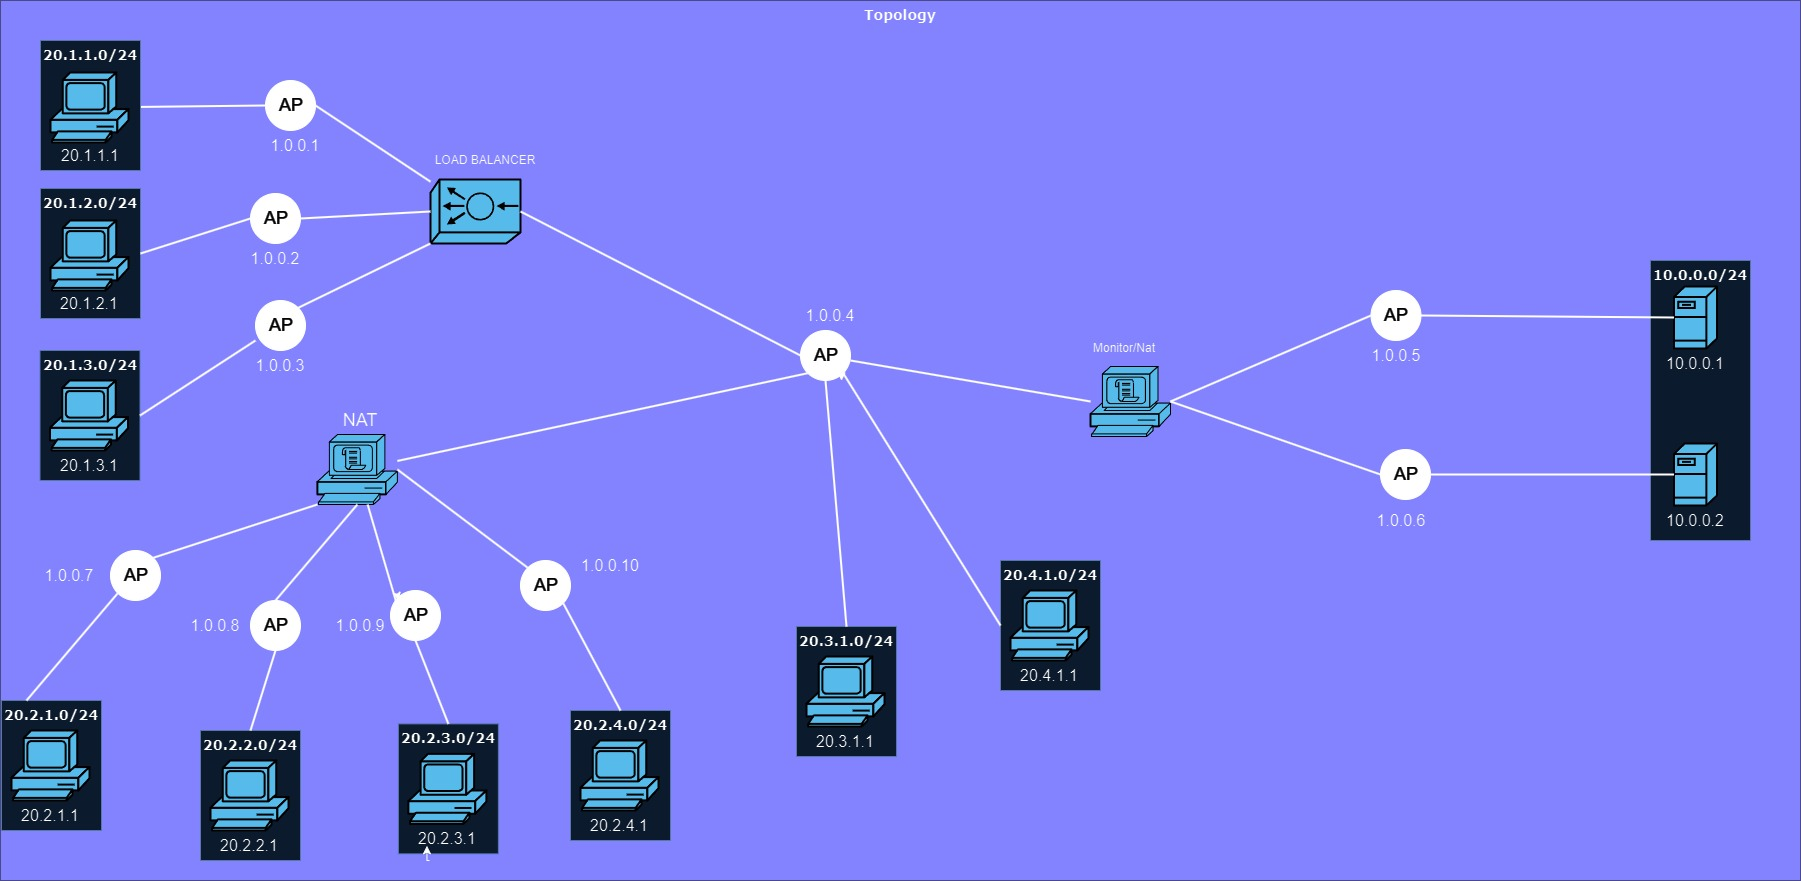
\includegraphics[width=1\textwidth]{Allocation_Graph.jpg} 
    \caption{Grafo di Allocazione della Demo B}
    \label{fig:AllocationGraphB}
\end{figure}

Entrando più nel dettaglio è possibile notare diversi gruppi di host, che rappresentano delle ipotetiche sedi aziendali separate. La prima, in alto a sinistra, viene descritta con la sottorete 20.1.0.0/16. All'interno di questo cluster sono presenti 
tre sottoreti rappresentate dagli ip 20.1.1.0/24, 20.1.2.0/24, 20.1.3.0/24. Le comunicazioni di queste sottoreti vengono regolate da un Load Balancer, che in caso di congestione del traffico decide arbitrariamente in quale nodo della rete inoltrare il traffico
per decongestionare alcuni collegamenti. La seconda sede aziendale è rappresentata in basso a sinistra dalla rete 20.2.0.0/16. Come per la prima sede sono presenti 4 sottoreti di host definite dagli ip 20.2.1.0/24, 20.2.2.0/24, 20.2.3.0/24, 20.2.4.0/24. Diversamente dalla 
prima, all'esterno del cluster 20.2.0.0/16 è presente un NAT che si occupa di mascherare gli indirizzi ip all'interno della rete con il resto della topologia. In basso sono inoltre presenti altre due sedi più piccole delle precedenti, definite dalle sottoreti 20.3.1.0/24 
e 20.4.1.0/24, queste dovrebbero simulare eventuali dipendenti in smart working che quindi non si connettono da una grande rete aziendale ma dalla propria rete di casa privata.\\
Sulla destra è invece presente una Server Farm definita dalla rete 10.0.0.0/24; all'interno sono stati definiti due Web Server con IP 10.0.0.1 e 10.0.0.2.  Infine è presente un nodo che funge da monitor (Mnt) per ispezionare il traffico in entrata ed uscita dai Web Server.
La topologia appena descritta può essere sintetizzata dalla tabella seguente:
\begin{table}
    \centering
    \begin{tabular}{ccc}
        \hline
         Name & IP & Functionality \\
        \hline
        C1-1 & 20.1.1.1 & Web Client behind load balancer \\
        C1-2 & 20.1.2.1 & Web Client behind load balancer \\
        C1-3 & 20.1.3.1 & Web Client behind load balancer \\
        Lb & 33.33.33.1 & Load balancer \\ 
        C2-1 & 20.2.1.1 & Web Client behind NAT \\
        C2-2 & 20.2.2.1 & Web Client behind NAT \\
        C2-3 & 20.2.3.1 & Web Client behind NAT \\
        C2-4 & 20.2.4.1 & Web Client behind NAT \\
        FW1 & 33.33.33.3 & Forwarder \\
        C3-1 & 20.3.1.1 & Web Client \\
        C4-1 & 20.4.1.1 & Web Client \\
        Mnt & 33.33.33.2 & Traffic Monitor \\
        S1 & 10.0.0.1 & Web Server \\
        S2 & 10.0.0.2 & Web Server \\
        \hline
    \end{tabular}
    \caption{Definizione nodi della topologia per Demo B}
    \label{tab:tabella}
\end{table}

Entrambi i server sono i punti d'interesse più importanti della topologia perchè le comunicazioni che verranno effettuate durante la simulazione utilizzeranno come 
uno dei due host almeno uno dei due server. Entrando più nello specifico l'obiettivo dei requisiti di sicurezza di isolamento e raggiungibilità sarà quello di rendere le 
comunicazioni della prima sede possibili solo con il server 10.0.0.2, della seconda sede solo con il server di 10.0.0.1 e delle restanti due sedi con entrambi i server. Per quanto riguarda
invece i requisiti di protezione l'obiettivo che si ci si è prefissati è quello di inserire almeno 2 VPN Gateway affinchè un host specifico all'interno della rete possa comunicare in maniera
sicura con i server per lo scambio di informazioni riservate. Di conseguenza è stato scelto uno degli host della prima sede, immaginandosi quindi la rete 20.1.0.0/16 come la sede centrale dell'azienda.
La definizione dei requisiti di sicurezza è quindi definibile in input al framework tramite la seguente tabella:

\begin{table}[H]
    \centering
    \small
    \setlength{\tabcolsep}{2pt} % Riduci il padding delle colonne
   \begin{tabular}{ccccccccc}
        \hline
         Policy & IPSrc & IPDst & pSrc & pDst & tProto & Confidentiality & Intregrity & Untrusted nodes\\
        \hline
        Isolation & 20.1.1.1 & 10.0.0.1 & * & * & ANY & // & // & // \\
        Reachability & 20.1.1.1 & 10.0.0.2 & * & * & ANY & // & // & // \\
        \hline
        Isolation & 20.1.2.1 & 10.0.0.1 & * & * & ANY & // & // & // \\
        Reachability & 20.1.2.1 & 10.0.0.2 & * & * & ANY & // & // & // \\
        \hline
        Isolation & 20.1.3.1 & 10.0.0.1 & * & * & ANY & // & // & // \\
        Reachability & 20.1.3.1 & 10.0.0.2 & * & * & ANY & // & // & // \\
        \hline
        Reachability & 20.2.1.1 & 10.0.0.1 & * & * & ANY & // & // & // \\
        Isolation & 20.2.1.1 & 10.0.0.2 & * & * & ANY & // & // & // \\
        \hline
        Reachability & 20.2.2.1 & 10.0.0.1 & * & * & ANY & // & // & // \\
        Isolation & 20.2.2.1 & 10.0.0.2 & * & * & ANY & // & // & // \\
        \hline
        Reachability & 20.2.3.1 & 10.0.0.1 & * & * & ANY & // & // & // \\
        Isolation & 20.2.3.1 & 10.0.0.2 & * & * & ANY & // & // & // \\
        \hline
        Reachability & 20.2.4.1 & 10.0.0.1 & * & * & ANY & // & // & // \\
        Isolation & 20.2.4.1 & 10.0.0.2 & * & * & ANY & // & // & // \\
        \hline
        Reachability & 20.3.1.1 & 10.0.0.1 & * & * & ANY & // & // & // \\
        Reachability & 20.3.1.1 & 10.0.0.2 & * & * & ANY & // & // & // \\
        \hline
        Reachability & 20.4.1.1 & 10.0.0.1 & * & * & ANY & // & // & // \\
        Reachability & 20.4.1.1 & 10.0.0.2 & * & * & ANY & // & // & // \\
        \hline
        Protection & 20.1.1.1 & 10.0.0.2 & * & 22 & ANY & AES-256-CBC & SHA2-256 & 33.33.33.2 \\
        \hline
    \end{tabular}
    \caption{Definizione requisiti di sicurezza della topologia per Demo B}
    \label{tab:tabellaNodiB}
\end{table}

\begin{itemize}
    \item \textbf{Prima coppia di Regole}: Il Web Client C1-1 deve poter essere sempre in grado di raggiungere con almeno un percorso il server S2 e non deve poter raggiungere con alcun percorso il server S1 all'interno della topologia. Per entrambe le regole non ci sono limitazioni di utilizzo sulla porta e sul protocollo di quarto livello, è quindi possibile utilizzare una qualsiasi porta nel range [0-65536] sia per il traffico in entrata che in uscita ed un protocollo a scelta fra UDP e TCP.
    \item \textbf{Seconda coppia di Regole}: Il Web Client C1-2 deve poter essere sempre in grado di raggiungere con almeno un percorso il server S2 e non deve poter raggiungere con alcun percorso il server S1 all'interno della topologia. Per entrambe le regole non ci sono limitazioni di utilizzo sulla porta e sul protocollo di quarto livello, è quindi possibile utilizzare una qualsiasi porta nel range [0-65536] sia per il traffico in entrata che in uscita ed un protocollo a scelta fra UDP e TCP. 
    \item \textbf{Terza coppia di Regole}: Il Web Client C1-1 deve poter essere sempre in grado di raggiungere con almeno un percorso il server S2 e non deve poter raggiungere con alcun percorso il server S1 all'interno della topologia. Per entrambe le regole non ci sono limitazioni di utilizzo sulla porta e sul protocollo di quarto livello, è quindi possibile utilizzare una qualsiasi porta nel range [0-65536] sia per il traffico in entrata che in uscita ed un protocollo a scelta fra UDP e TCP.
    \item \textbf{Quarta coppia di Regole}: Il Web Client C2-1 deve poter essere sempre in grado di raggiungere con almeno un percorso il server S1 e non deve poter raggiungere con alcun percorso il server S2 all'interno della topologia. Per entrambe le regole non ci sono limitazioni di utilizzo sulla porta e sul protocollo di quarto livello, è quindi possibile utilizzare una qualsiasi porta nel range [0-65536] sia per il traffico in entrata che in uscita ed un protocollo a scelta fra UDP e TCP.
    \item \textbf{Quinta coppia di Regole}: Il Web Client C2-2 deve poter essere sempre in grado di raggiungere con almeno un percorso il server S1 e non deve poter raggiungere con alcun percorso il server S2 all'interno della topologia. Per entrambe le regole non ci sono limitazioni di utilizzo sulla porta e sul protocollo di quarto livello, è quindi possibile utilizzare una qualsiasi porta nel range [0-65536] sia per il traffico in entrata che in uscita ed un protocollo a scelta fra UDP e TCP.
    \item \textbf{Sesta coppia di Regole}: Il Web Client C2-3 deve poter essere sempre in grado di raggiungere con almeno un percorso il server S1 e non deve poter raggiungere con alcun percorso il server S2 all'interno della topologia. Per entrambe le regole non ci sono limitazioni di utilizzo sulla porta e sul protocollo di quarto livello, è quindi possibile utilizzare una qualsiasi porta nel range [0-65536] sia per il traffico in entrata che in uscita ed un protocollo a scelta fra UDP e TCP.
    \item \textbf{Settima coppia di Regole}: Il Web Client C2-4 deve poter essere sempre in grado di raggiungere con almeno un percorso il server S1 e non deve poter raggiungere con alcun percorso il server S2 all'interno della topologia. Per entrambe le regole non ci sono limitazioni di utilizzo sulla porta e sul protocollo di quarto livello, è quindi possibile utilizzare una qualsiasi porta nel range [0-65536] sia per il traffico in entrata che in uscita ed un protocollo a scelta fra UDP e TCP.
    \item \textbf{Ottava coppia di Regole}: Il Web Client C3-1 deve poter essere sempre in grado di raggiungere con almeno un percorso il server S1 e con almeno un percorso anche il server S2. Per entrambe le regole non ci sono limitazioni di utilizzo sulla porta e sul protocollo di quarto livello, è quindi possibile utilizzare una qualsiasi porta nel range [0-65536] sia per il traffico in entrata che in uscita ed un protocollo a scelta fra UDP e TCP.
    \item \textbf{Nona coppia di Regole}: Il Web Client C4-1 deve poter essere sempre in grado di raggiungere con almeno un percorso il server S1 e con almeno un percorso anche il server S2. Per entrambe le regole non ci sono limitazioni di utilizzo sulla porta e sul protocollo di quarto livello, è quindi possibile utilizzare una qualsiasi porta nel range [0-65536] sia per il traffico in entrata che in uscita ed un protocollo a scelta fra UDP e TCP.
    \item \textbf{Decima Regola}: Il Web Client C1-1 deve poter comunicare in maniera sicura con il Web Server S2. Il traffico originato da C1-1 può utilizzare qualsiasi porta di uscita per il protocollo di trasporto ma il Server S2 deve ricevere i dati in ingresso unicamente dalla porta 22. È possibile utilizzare sia il protocollo UDP che TCP per il trasporto. Viene specificato infine il nodo Mnt come nodo non sicuro e attraverso il quale il traffico deve passare cifrato.
\end{itemize}

Come ampiamente è stato già discusso per la Demo A, anche in questo caso non è sufficiente definire le regole su Verefoo per assicurarsi di avere una soluzione ottimale, ma è necessario creare un ambiente isolato in grado di testare la correttezza delle configurazioni prodotte da Verefoo. Anche in questo caso è stato scelto
di utilizzare Docker Compose per la realizzazione di una rete virtuale, nella quale ogni host, server, forwarder, firewall e VPN gateway è rappresentato univocamente da un container in esecuzione. Di seguito viene presentata una parte dei servizi definiti all'interno del docker-compose file per istanziare una topologia del genere:

\begin{lstlisting}[style=yaml,caption={Definizione di Services dell'ambiente virtuale DemoB},label=composeDemoA]
    server1:
    container_name: server1
    hostname: server1
    image: endpoint
    cap_add:
      - NET_ADMIN
    command: >-
      sh -c "route del default && route add -net 0.0.0.0 netmask 0.0.0.0 gw
      10.0.0.100 && tail -F anything"
    networks:
      servers:
        ipv4_address: 10.0.0.1
  server2:
    container_name: server2
    hostname: server2
    image: endpoint
    cap_add:
      - NET_ADMIN
    command: >-
      sh -c "route del default && route add -net 0.0.0.0 netmask 0.0.0.0 gw
      10.0.0.199 && tail -F anything"
    networks:
      servers:
        ipv4_address: 10.0.0.2

   forwarder1:
     container_name: forwarder1
     hostname: forwarder1
     image: endpoint
     cap_add:
        - NET_ADMIN
     volumes:
        - './RouterVPNConfig:/mnt:ro'
     command: sh -c "/mnt/staticroutes/forone && tail -F anything"
     networks:
        servers:
            ipv4_address: 10.0.0.100
          forwarder1_vpn3:
            ipv4_address: 130.0.3.2
          forwarder1_fw: 
            ipv4_address: 80.0.1.2
   client1_1:
            container_name: client1_1
            hostname: client1_1
            image: endpoint
            cap_add:
              - NET_ADMIN
            command: >-
              sh -c "route del default && route add -net 0.0.0.0 netmask 0.0.0.0 gw
              20.1.1.100 && tail -F anything"
            networks:
              clients1_1:
                ipv4_address: 20.1.1.1
    
\end{lstlisting}


In questo design, diversamente dal precedente, è possibile notare come i due Web Server condividono la stessa rete, ma viene impostato un default gateway differente. Questa scelta è stata necessaria in quanto 
come è possibile notare nella figura (\ref{fig:AllocationGraphB}) sono presenti due diversi allocation place per collegare i due elementi. Grazie a questa configurazione sarà quindi possibile instanziare Network Security Functions
differenti a seconda del server con cui si comunica. Nelle definizioni d'esempio è presente pure quella di un forwarder, in questo caso seppur l'immagine utilizzata per la costruzione del container è identica a quella di un endpoint generico
durante l'instanziazione del container viene eseguito un comando bash aggiuntivo che carica il file "forone" dalle static route. Tramite ciò è possibile definire tutti i forwarding path per ogni elemento che non influenza le proprietà di sicurezza della rete.\\
Per quanto riguarda i Web Client all'interno della topologia la singola definizione è identica a quella proposta all'interno della Demo A con l'unica maggiore differenza è che è stato scelto l'ip terminante con \textit{".100"} come il default gateway per ogni 
host.\\ \\ 
Entrando più nello specifico, è stato necessario definire delle immagini dalle quali istanziare i container grazie al Docker deamon. Per tutte le immagini si è deciso di utilizzare delle immagini di alpine, una distribuzione Linux estremamente leggera in termini di dimensioni su disco e generalmente sicura, nella quale sono poi installabili eventuali
package aggiuntivi che permettono di creare delle versioni custom dell'immagine a seconda di ciò che vogliamo far svolgere al container. Nel caso degli endpoint la definizione del Dockerfile è la seguente:


\begin{lstlisting}[style=bashstyle, caption={Definizione Dockerfile Endpoint}, label=lst:bash-dockerfileEnd,numbers=left]
    FROM alpine:latest

    RUN apk update
    RUN apk add hping3 --update-cache --repository http://dl-cdn.alpinelinux.org/alpine/edge/testing
    RUN apk add tcpdump
    RUN apk add  net-tools 
    ENV PS1='\h:\w\$ '
    
    CMD ["/bin/sh"];
\end{lstlisting}

Partendo dall'ultima immagine disponibile nel repository generale di Docker viene installato un container alpine, successivamente viene fatto un update dei vari package disponibili e installato il package hping3 che consente di inviare dei pacchetti ICMP/UDP/TCP
e tracciare il loro percorso all'interno della rete utilizzando il comando \textit{"--traceroute"}. Questo package è  puramente necessario per eseguire le operazioni di debug e controllo all'interno della rete. Completano il container i package tcpdump e net-tools
che permettono rispettivamente di osservare le interfacce di rete per osservare i pacchetti in transito e di eseguire comandi per la configurazione di rete come ifconfig, arp. ipmaddr eccetera.\\

Nonostante gli output non siano ancora stati prodotti, dai requisiti di sicurezza ci si aspetta di avere degli allocation places nel quale verranno istanziati Firewall e VPN. Di conseguenza dei Dockerfile sono stati scritti per la futura allocazione di queste Security Network Functions.
Di seguito viene fornito il Dockerfile dei container destinati a diventare Firewall:
\begin{lstlisting}[style=bashstyle, caption={Definizione Dockerfile Firewall}, label=lst:bash-dockerfileEnd,numbers=left]
    FROM alpine:latest

    RUN apk update
    RUN apk add iptables sudo
    RUN apk add tcpdump
    RUN apk add bash
    RUN apk add --no-cache quagga \
     && touch /etc/quagga/zebra.conf \
     && touch /etc/quagga/vtysh.conf \
     && touch /etc/quagga/ripd.conf
    ENV PS1='\h:\w\$ '     
    CMD ["/bin/sh"];
\end{lstlisting}
All'interno di questa configurazione di alpine viene installato il package iptables, che è necessario in quanto permette di definire a livello software un firewall, di monitorare il traffico in ingresso ed uscita dal nodo e di scartare 
eventuali pacchetti che non soddisfano la configurazione. A questo package si aggiunge quagga che è un package in grado di definire delle funzioni di routing avanzate per comunicazioni basate su TCP o IP. All'interno della cartella di installazione di quagga vengono
poi definiti dei file di configurazione necessari ad un corretto funzionamento del software. I packages di tcpdump e bash sono presenti solamente per effettuare operazioni di debug e test.\\

Infine è disponibile una definizione dell'immagine di un ipotetico VPN Gateway:
\begin{lstlisting}[style=bashstyle, caption={Definizione Dockerfile VPN Gateway}, label=lst:bash-dockerfileEnd,numbers=left]
    FROM alpine:latest
    RUN apk update
    RUN apk add  net-tools 
    RUN apk add iptables sudo
    RUN apk add tcpdump
    RUN apk add --update strongswan && \
        rm -rf /var/cache/apk/* && \
        mkdir -p /etc/strongswan
    ENV PS1='\h:\w\$ ' 
    CMD ["/bin/sh"]
\end{lstlisting}

Quest'ultima configurazione oltre ad utilizzare alcuni packages come iptables, tcpdump e net-tools discussi precedentemente installa il software fondamentale per effettuare operazioni di tunneling VPN ovvero strongswan. Questo package è in grado di accettare
le configurazioni che vengono fornite in output dal Translator di Verefoo, velocizzando quindi le operazioni di testing delle configurazioni prodotte.

\section{Output}
\subsection{Topologia di Rete}
Una volta definito tutto il necessario affinchè sia possibile istanziare in sicurezza e in maniera corretta un ambiente virtuale basato sui container Docker, è possibile iniziare a verificare la correttezza della nuova versione del framework analizzando i suoi output.
È importante sottolineare che il numero di allocation places definiti in input è volutamente inferiore a quello necessario per rispettare i vincoli in maniera ottimale. Tramite questa scelta di design è quindi possibile controllare che i nuovi allocation places istanziati dopo 
l'allocazione delle VPN vengano considerati nel calcolo delle soluzioni ottimali.\\
Fornendo quindi l'output definito nel paragrafo precedente la soluzione prodotta in output da Verefoo è la seguente:

\begin{figure}[h]  % 'h' significa che la figura viene posizionata qui
    \centering
    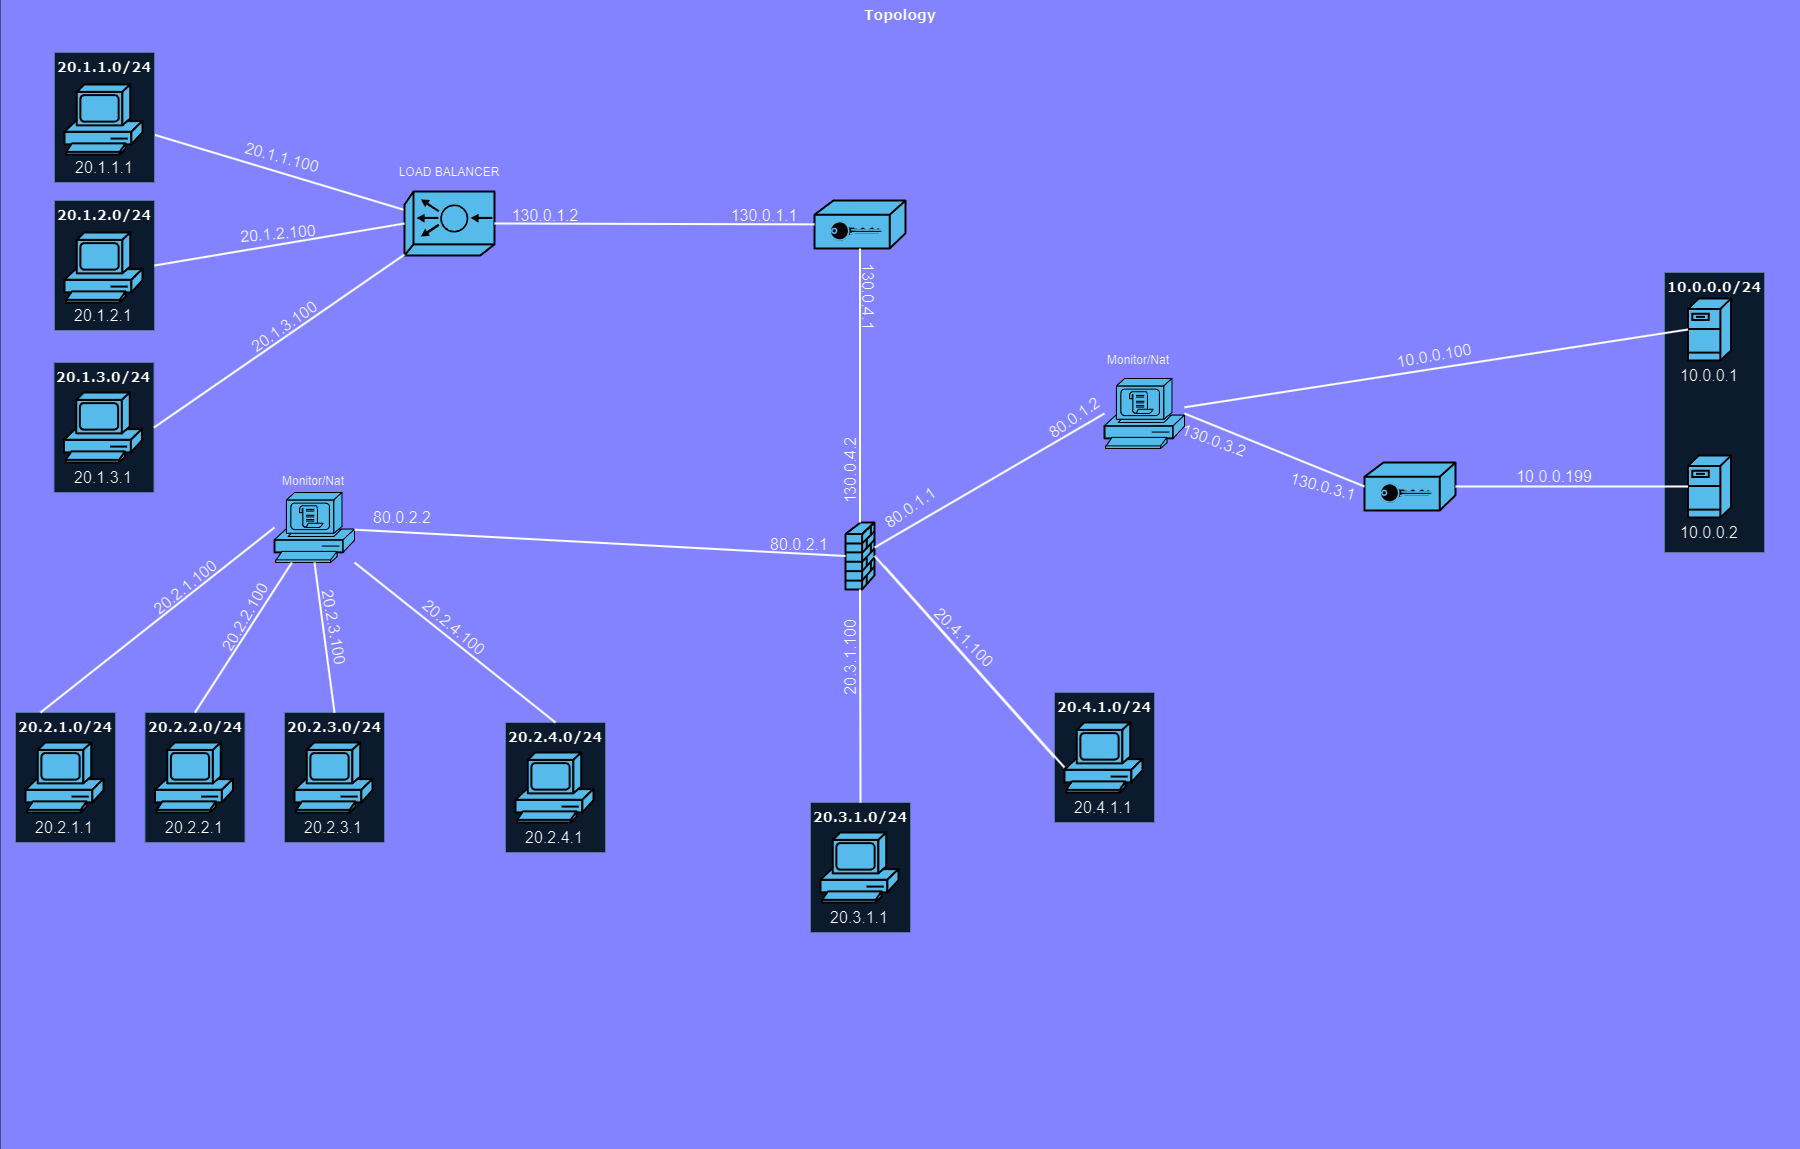
\includegraphics[width=1\textwidth]{Topologia_finale.png} 
    \caption{Verefoo Output}
    \label{fig:VPNDeploy}
\end{figure}

Come ci si poteva aspettare, dati i requisiti di sicurezza definiti sono state allocate tre Network Security Functions. Al centro della topologia è stato inserito un Firewall, che a prima vista sembra essere posizionato correttamente perchè in quella posizione riesce a scartare il traffico proveniente sia dalla
rete 20.1.*.*/16 che quello dalla rete 20.2.*.*/16. Ai lati sinistro e destro sono invece presenti i due VPN Gateway, occorre portare particolare attenzione a quello situato a sinistra in quanto il suo allocation places non era presente in input (figura \ref{fig:AllocationGraphB}), di conseguenza è possibile dedurre che dopo aver
istanziato una Network Security Function la successiva è stata posizionata in uno degli allocation places aggiuntivi formati nella nuova versione del framework.

\subsection{Configurazioni Network Security Functions}
Data la posizione che sembra definire una soluzione plausibilmente corretta, è possibile analizzare anche le configurazioni fornite per ogni funzione di sicurezza.
La seguente è la tabella che descrive la configurazione dei due gateway VPN:

\begin{table}[H]
    \centering
    \begin{tabular}{ccccccc}
        \hline
         Name & Action & IPSrc & IPDst & pSrc & pDst & tProto \\
        \hline
        VPN1 & ACCESS & 20.1.1.1 & 10.0.0.2 & * & 22 & ANY \\
        VPN2 & EXIT & 20.1.1.1 & 10.0.0.2 & * & 22 & ANY \\
        \hline
    \end{tabular}
    \caption{Configurazione dei due VPN gateway Demo B}
    \label{tab:tabella}
\end{table}

Come si può notare, dato l'unico requisito di protezione che era stato definito, solo due gateway sono stati allocati, rispettivamente di accesso per quanto riguarda il gateway presente a sinistra, e di uscita per quello di destra.
In entrambe le configurazioni si può notare che il singolo host dal quale comunicazioni dovranno essere cifrate è la sorgente 20.1.1.1, mentre il nodo di destinazione è il server S2 definito dall'IP 10.0.0.2. Anche i requisiti sul protocollo di trasporto
sono verificati in quanto la porta di destinazione che il server deve ricevere è la 22 che è quella indicata nei requisiti ed inoltre anche nella configurazione non c'è nessun vincolo di protocollo tra TCP e UDP.\\
Per quanto riguarda invece la configurazione del firewall, Verefoo fornisce il seguente output:

\begin{table}[H]
    \centering
    \begin{tabular}{ccccccc}
        \hline
        Default Action & Action & IPSrc & IPDst & pSrc & pDst & tProto \\
        \hline
        ALLOW & DENY & 20.1.*.* & 10.0.0.1 & * & * & ANY \\
        ALLOW & DENY & 20.2.*.* & 10.0.0.2 & * & * & ANY  \\
        \hline
    \end{tabular}
    \caption{Configurazione Firewall Demo B}
    \label{tab:tabella}
\end{table}

Anche in questo caso il framework sembra produrre una soluzione plausibile, in quanto il Firewall è stato configurato in blacklist, permettendo a qualsiasi traffico il transito tranne a quello 
definito nelle regole specifiche del firewall. In questo modo è possibile far comunicare tranquillamente le sottoreti 20.3.1.0/24 e 20.4.1.0/24 in quanto qualsiasi pacchetto da e per i due server S1 ed S2 non verrà
mai scartato dal firewall. Viceversa per quanto riguarda le sottoreti 20.1.0.0/16 e 20.2.0.0/16 il framework non solo ha prodotto delle regole corrette, ma è riuscito anche a raggruppare tutte le definizioni singole sulle reti più piccole in una
definizione più generale grazie alla notazione con \textit{"*"}. Tramite ciò quindi ogni elemento appartenente alla sottorete 20.1.0.0/16 non potrà comunicare con il server S1 ed ogni elemento nella rete 20.2.0.0/16 non potrà comunicare con il server S2.

\subsection{Configurazioni Strongswan}
Nonostante le configurazioni della topologia e delle network security function siano corrette, il framework prodotto allo stato attuale non fornisce una implementazione aggiornata del Translator di Strongswan, non è quindi possibile ottenere automaticamente 
una versione aggiornata dei file di configurazione "swanctl.conf". Per aggirare questo problema, durante lo sviluppo di questa Demo i file di configurazione dei due Gateway sono stati prodotti manualmente a partire dalle configurazioni fornite da Verefoo. \\
Di conseguenza, il seguente snippet di codice rappresenta uno dei due file di configurazione scritti per testare l'ambiente virtuale:

\begin{lstlisting}[language=sh]
    connections {
   site-site {
      local_addrs  = 130.0.4.1
      remote_addrs = 130.0.3.1
      local {
         auth = pubkey
         certs = VpnConfig1Cert.pem
         id = VpnConfig1.strongswan.org
      }
      remote {
         auth = pubkey
         id = VpnConfig2.strongswan.org
      }
      children {
         net-net {
            local_ts = 20.1.1.1/32            
            remote_ts = 10.0.0.2/32            
            start_action = trap|start 
            rekey_time = 5400
            rekey_bytes = 500000000
            rekey_packets = 1000000
            esp_proposals = aes256-sha2_256-modp2048
         }
      }
      version = 2
      mobike = no
      reauth_time = 10800
   }
   
}
\end{lstlisting}

All'interno di questo esempio la connessione site-to-site è definita dalle interfacce dei due VPN gateway con IP 130.0.4.1 e 130.0.3.1. In locale vengono caricati i certificati attraverso
il file VpnConfig1Cert.pem e l'autenticazione viene effettuata tramite chiave pubblica asimmetrica, in maniera simile viene definito l'id e il metodo di autenticazione del gateway remoto.
Infine viene dichiarata una connessione end-to-end tra il client C1-1 definito da 20.1.1.1/32 e il Web Server S2 definito da 10.0.0.2/32. All'interno di questa connessione viene definita anche la proposta
da effettuare per l'incapsulamento in IPSec tramite il protocollo ESP, utilizzando gli algoritmi di aes256-cbc e sha2-256.

\section{Verifiche e Test}

Grazie alle configurazioni prodotte in output dalla nuova versione del framework è possibile verificare che le soluzioni prodotte siano efficaci e corrette.
Per fare ciò, come nella demo precedente è stato predisposto un ambiente virtuale composto da container Docker che simuleranno il comportamento di ogni elemento di rete descritto nella topologia. In questo caso
le verifiche da effettuare all'interno della topologia saranno diverse perchè non sarà necessario dimostrare solo che le comunicazioni fra l'host C1-1 ed il server S2 siano protette tramite crittografia ma è anche
necessario controllare se le comunicazioni fra i client ed i vari host vengono filtrate dal firewall. \\
Partendo dalla verifica del firewall sarà necessario utilizzare due terminali differenti, il primo corrispondente al client C1-1 che come da requisiti dovrebbe essere in grado di comunicare solo con il server S2, isolando tutte le
comunicazioni con S1. Per testare ciò utilizzeremo i seguenti comandi Linux:

\begin{figure}[H] 
    \centering
    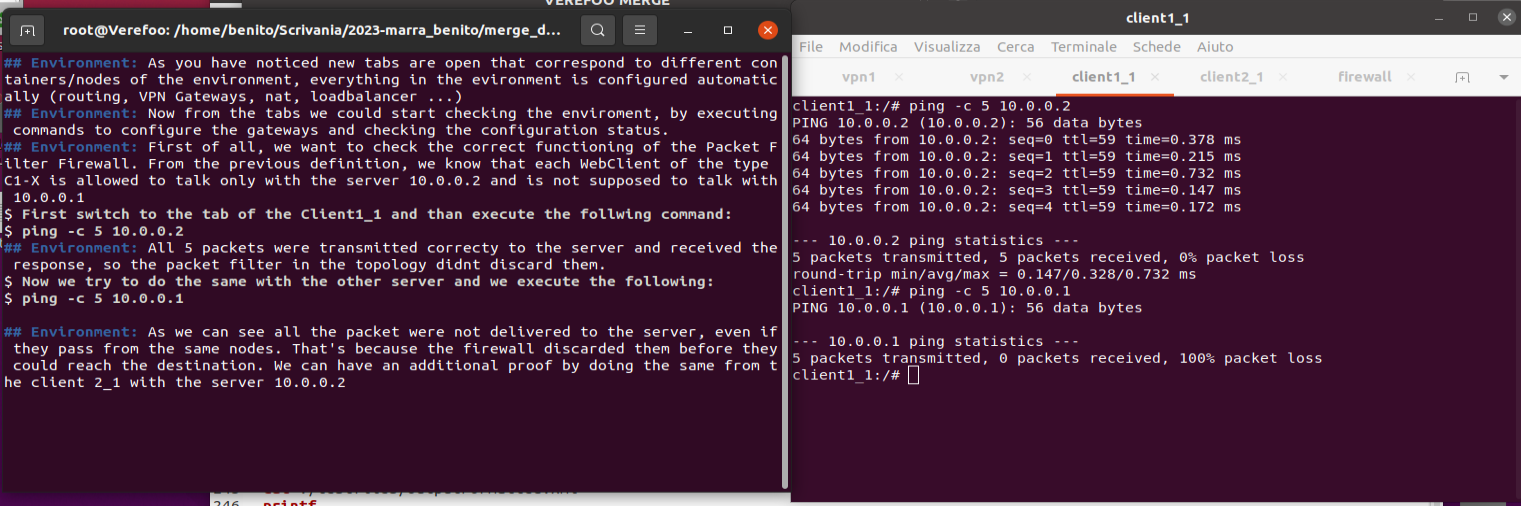
\includegraphics[width=1\textwidth]{(1)FirewallDiscard1.png} 
    \caption{Verifica pacchetti scartati dal Firewall per rete 20.1.*.*}
    \label{fig:Verifica1}
\end{figure}

All'interno del terminale C1-1 eseguiamo il comando \textit{"ping -c 5 [ipaddr]"} per verificare le connessioni con i due server presi in esame.
Nel primo caso testiamo sul server dall'IP "10.0.0.2" ovvero S2: come si può notare vengono trasferiti 5 pacchetti col protocollo ICMP e contemporaneamente vengono
ricevuti 5 pacchetti con una statistica di 0\% packet loss. Se invece eseguiamo la stessa operazione con il server dall'IP "10.0.0.1" il risultato sarà opposto, ovvero tutti
i pacchetti inviati vengono scartati non ricevendo alcuna risposta ed il numero di packet loss sarà uguale al 100\%.\\
Considerando il percorso che eseguono i pacchetti, ovvero\\
 $ \text{C1-1} \rightarrow \text{Lb} \rightarrow \text{VPNGateway1} \rightarrow \text{Firewall} \rightarrow \text{Monitor} \rightarrow \text{VPNGateway2} \rightarrow \text{Server}$
è possibile dedurre che l'elemento che scarta i pacchetti e impedisce le comunicazioni è proprio il firewall con la configurazione prodotta da Verefoo.\\
Tuttavia verificare le comunicazioni fra il client C1-1 ed il Server S2 non è sufficiente a verificare il corretto funzionamento del firewall, è infatti necessario assicurarsi che anche
le comunicazioni all'interno della rete 20.2.0.0/16 vengano filtrate quando si prova a comunicare con il server S1. 
\begin{figure}[H] 
    \centering
    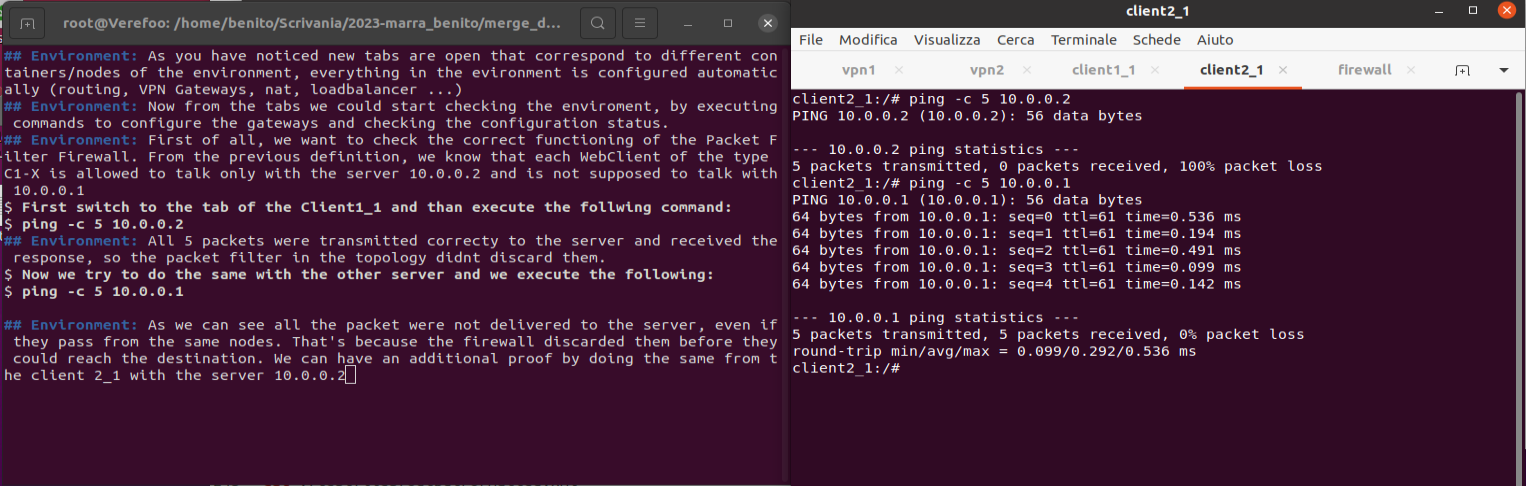
\includegraphics[width=1\textwidth]{(2)FirewallDiscard2.png} 
    \caption{Verifica pacchetti scartati dal Firewall per rete 20.2.*.*}
    \label{fig:Verifica2}
\end{figure}

Per verificare anche questa condizione vengono effettuati gli stessi comandi sul terminale del client C2-1, avendo un IP appartenente alla rete 20.2.0.0/16.
Il risultato che viene visualizzato in output è coerente con quello che ci si aspetta, essendo opposto all'output del client C1-1. Le comunicazioni con il server
10.0.0.2 non risultano possibili in quanto ogni pacchetto è stato scartato dal Firewall ed è presente anche qua il 100\% di packet loss, viceversa quando si fa un ping 
sul server 10.0.0.1 corrispondente a S1 ogni pacchetto viene correttamente trasmesso e ricevuto dal server, passando quindi i controlli del firewall. \\
È quindi possibile affermare che le configurazioni riguardanti i requisiti di raggiungibilità e di isolamento prodotte dal framework risultano corrette e con il minimo uso 
di risorse possibili, in quanto grazie ad un unico firewall sono state soddisfatte tutte le caratteristiche fornite in input. \\ \\
La successiva verifica che deve essere effettuata sulla bontà della soluzione prodotta riguarda l'istanziazione e la configurazione dei VPN Gateway nella topologia di output.
In questa istanza specifica solo 2 gateway sono stati allocati, quindi è sufficiente verificare che i pacchetti in transito tra il nodo C1-1 ed il server S2 risultano cifrati
correttamente. Prendendo spunto dai test effettuati nella demo precedente utilizziamo tcpdump nel seguente modo:

\begin{figure}[H] 
    \centering
    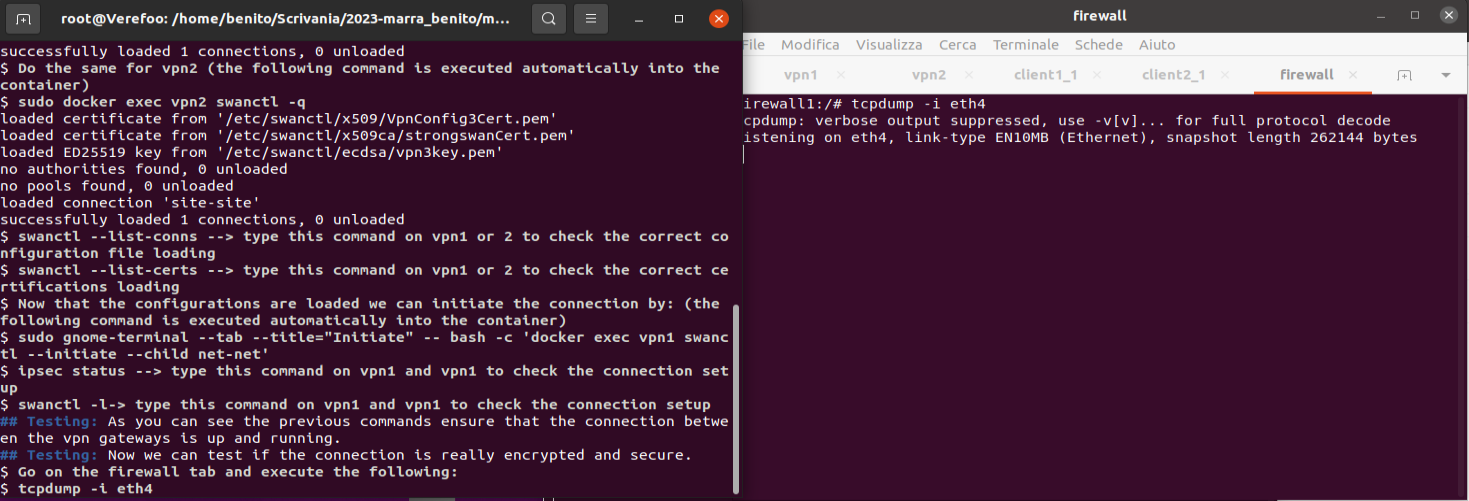
\includegraphics[width=1\textwidth]{(3)Firewall_tcpdump_setup.png} 
    \caption{Setup tcpdump per verifiche di sicurezza}
    \label{fig:Verifica3}
\end{figure}

Il nodo preso in analisi è lo stesso in cui viene instanziato il firewall, utilizzando tcpdump è possibile  osservare e monitorare i pacchetti in transito attraverso una delle interfacce
del nodo. L'interfaccia scelta per questo test è "eth4" corrispondente alla connessione fra il firewall ed il primo VPN Gateway. Il risultato aspettato è quindi, come per la prima demo, osservare
il transito dei pacchetti non come semplici ICMP packets ma come ESP packets, ovvero il protocollo utilizzato per l'incapsulamento in IPsec.\\
Per controllare l'output è quindi necessario, una volta impostato il monitoraggio dell'interfaccia, eseguire il comando di ping come fatto per il firewall precedentemente e controllare l'output 
nel terminale del firewall. Di seguito viene proposto un possibile output effettuato: 


\begin{figure}[H] 
    \centering
    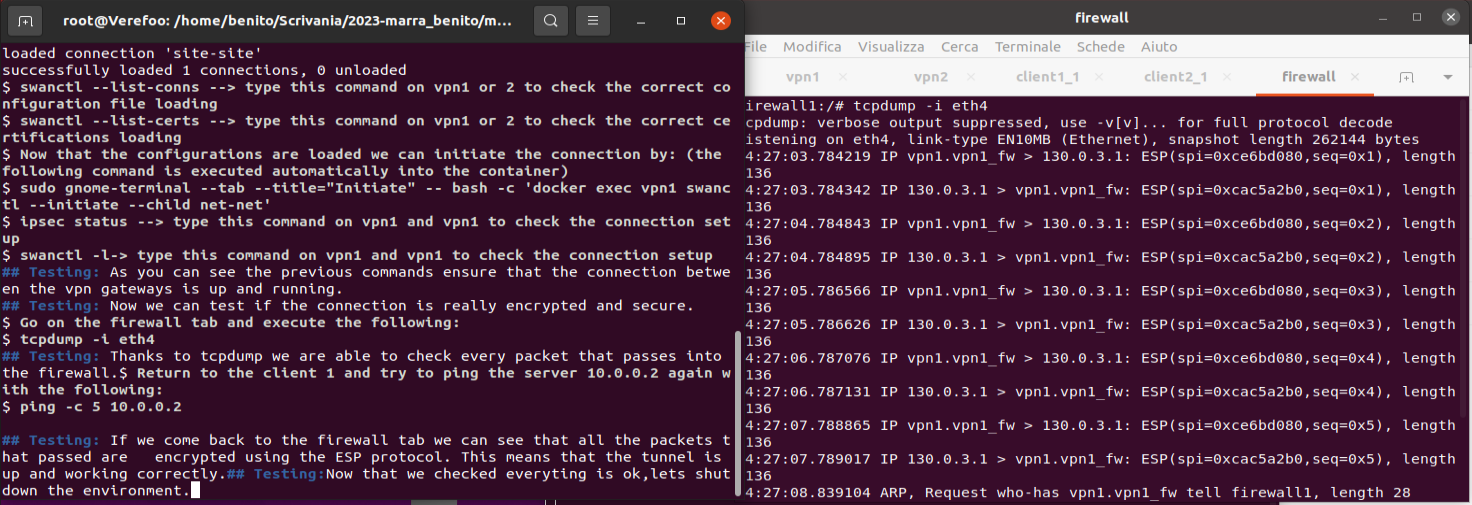
\includegraphics[width=1\textwidth]{(4)Encryptedpacket_output.png} 
    \caption{Verifica cifratura dei pacchetti in transito}
    \label{fig:Verifica4}
\end{figure}

Il risultato ottenuto corrisponde alle aspettative descritte precedentemente. È infatti possibile notare come ogni pacchetto venga codificato con il protocollo ESP e venga monitorato con il path specifico del tunnel VPN.
Di conseguenza è possibile affermare che il risultato prodotto da Verefoo è corretto in quanto garantisce la sicurezza in tutto il traffico partente dal nodo C1-1 al server S2. Grazie a questa ennesima verifica anche i requisiti
di sicurezza sono rispettati, confermando la correttezza del framework e della demo prodotta. Di conseguenza si può affermare che anche il terzo ed ultimo obiettivo della tesi è stato portato a termine, producendo una demo funzionante che
mettesse in risalto le caratteristiche della nuova versione del framework.

